\def\year{2017}\relax
%File: formatting-instruction.tex
\documentclass[letterpaper]{article} %DO NOT CHANGE THIS
\usepackage{aaai19}  %Required
\usepackage{times}  %Required
\usepackage{helvet}  %Required
\usepackage{courier}  %Required
\usepackage{url}  %Required
\usepackage{graphicx}  %Required
\frenchspacing  %Required
\setlength{\pdfpagewidth}{8.5in}  %Required
\setlength{\pdfpageheight}{11in}  %Required
%PDF Info Is Required:
  \pdfinfo{}
\setcounter{secnumdepth}{0}

\usepackage{amsmath}
\usepackage{amssymb}
\usepackage{amsthm}
\usepackage{multirow}
\usepackage{tikz}
\usetikzlibrary{arrows,automata}
\usepackage{comment}

\usepackage{graphicx}
\usepackage{caption}
\usepackage{subcaption}
\usepackage{listings}

\lstset{
  basicstyle=\ttfamily,
  mathescape
}


\usepackage{multicol}
\usepackage{arydshln}
\usetikzlibrary{calc,backgrounds,positioning,fit}


\newcommand{\tup}[1]{{\langle #1 \rangle}}

\newcommand{\pre}{\mathsf{pre}}     % precondition
\newcommand{\del}{\mathsf{del}}     % effect
\newcommand{\add}{\mathsf{add}}     % effect
\newcommand{\eff}{\mathsf{eff}}     % effect
\newcommand{\cond}{\mathsf{cond}}   % conditional effect
\newcommand{\true}{\mathsf{true}}   % true
\newcommand{\false}{\mathsf{false}} % false
\newcommand{\PE}{\mathrm{PE}}     % precondition
\newcommand{\strips}{\textsc{Strips}}     % precondition


\newtheorem{theorem}{Theorem}
\newtheorem{lemma}[theorem]{Lemma}
\newtheorem{definition}[theorem]{Definition}


\begin{document}

\title{Model Recognition as Planning}

% Commented for blind submission
\author{Diego Aineto \and Sergio Jim\'enez\and Eva Onaindia\\
{\scriptsize Departamento de Sistemas Inform\'aticos y Computaci\'on}\\
{\scriptsize Universitat Polit\`ecnica de Val\`encia.}\\
{\scriptsize Camino de Vera s/n. 46022 Valencia, Spain}\\
{\scriptsize \{dieaigar,serjice,onaindia\}@dsic.upv.es}
\And Miquel Ram\'irez\\
{\scriptsize School of Computing and Information Systems}\\
{\scriptsize The University of Melbourne}\\
{\scriptsize Melbourne, Victoria. Australia}\\
{\scriptsize miquel.ramirez@nimelb.edu.au}}


\maketitle
\begin{abstract}
Given a partially observed plan execution, and a set of possible planning models (models that share the same state variables but different action models), {\em model recognition} is the task of identifying the model that explains the observation. The paper formalizes this task and introduces a novel method that estimates the probability of a \strips\ model to produce an observation of a plan execution. This method builds on top of off-the-shelf classical planning algorithms and it is robust to missing actions and intermediate states in the observation. The effectiveness of the method is tested in three experiments, each encoding a set of different \strips\ models and all using empty-action observations: (1) a classical string classification task; (2) identification of the model that encodes a failure present in an observation; and (3) recognition of a robot navigation policy.
\end{abstract}

\section{Introduction}
\label{sec:introduction}
{\em Plan recognition} is the task of predicting the future actions of an agent provided observations of its current behavior~\cite{Carberry01}. {\em Goal recognition} is a closely related task that aims identifying the goals of the observed agent. Goal recognition is considered {\em automated planning} in reverse; while automated planning compute sequences of actions that accounts for a given goals, goal recognition compute goals that account for an observed sequence of actions~\cite{geffner:book:2013}.

Diverse approaches has been proposed for plan/goal recognition such as {\em rule-based systems}, {\em parsing}, {\em graph-covering}, {\em Bayesian nets}, etc~\cite{sukthankar14}. {\em Plan recognition as planning} is the model-based approach for plan/goal recognition that leverages the action model of the observed agent to compute its most likely goal~\cite{ramirez2012plan,ramirez2009plan}.

This paper formalizes the {\em model recognition} task where the object to recognize is not a goal but the {\em planning model} that shapes the behavior of the observed agent. Given a partially observed plan execution, and a set of possible planning models (models that share the same state variables but that update these variables with different action models); {\em model recognition} is the task of identifying the model in the set with the highest probability of producing/explaining the given observation.

\begin{figure}
  \begin{scriptsize}
  \begin{center}
  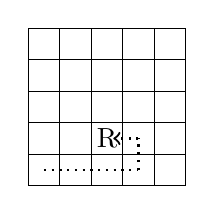
\begin{tikzpicture}[scale=.4]
          \begin{scope}
            \draw (0, 0) grid (5, 5);
            \node[anchor=center] at (2.5, 1.5) {R};
            \node[anchor=center] at (0.5, 0.5) {};
            \draw[thick,style=dotted] (0.5,0.5) -- (3.5,0.5);
            \draw[thick,style=dotted] (3.5,0.5) -- (3.5,1.5);
            \draw[thick,style=dotted,->] (3.5,1.5) -- (2.7,1.5);
          \end{scope}
        \end{tikzpicture}
\hspace*{1cm}
	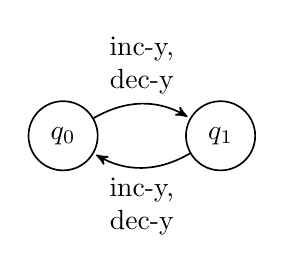
\begin{tikzpicture}[->,>=stealth',shorten >=1pt,auto,node distance=2cm,semithick]
	  \node[state] (A)              {$q_0$};
	  \node[state] (B) [right of=A] {$q_1$};
	  \path
(A) edge [bend left, align=center] node {inc-y,\\dec-y} (B)
(B) edge [bend left, align=center] node {inc-y,\\dec-y} (A);
	\end{tikzpicture}
  \end{center}
  \end{scriptsize}
 \caption{\small ({\em Left)} Robot navigating a $5\times 5$ grid. {\em (Right)} Automata to control that the robot only increments its x-coordinate when $q_0$ holds (actions {\tt inc-y} and {\tt dec-y} update the robot y-coordinate and switch the automata state).}
\label{fig:grid-example}
\end{figure}

To better illustrate {\em model recognition}, imagine a robot in a $N\times N$ grid whose navigation is determined by the \strips\ model of Figure~\ref{fig:model-example}. According to this model, the robot can increment its {\em x-coordinate} when {\tt\small $q0$} holds (i.e. at {\em even rows} if {\tt\small $q0$} holds initially) and decrement it when {\tt\small $q1$} holds (at {\em odd rows} if {\tt\small $q0$} holds initially). Apart from the model of Figure~\ref{fig:model-example}, different models can be defined within the same state variables (e.g. altering the way {\tt\small $q0$} and {\tt\small $q1$} are required and updated) and these models can shape different kinds of robot navigation. Given a partially observed plan execution (like the one illustrated at Figure~\ref{fig:grid-example} where state variables {\small\tt $q0$} and {\small\tt $q1$} are unobserved) {\em model recognition} aims to identify the action model that produced/explains that observation.

{\em Model recognition} is of interest because once the planning model is recognized, then the model-based machinery for automated planning becomes applicable~\cite{ghallab2004automated}. In addition, it enables identifying different kinds of automata by observing their execution. It is well-known that diverse automata representations, like {\em finite state controllers}, {\em B\"{u}chi automata}, {\em push-down automata}, {\em {\sc GOLOG} programs} or {\em reactive policies}, can be encoded as classical planning models~\cite{BaierFM07,Geffner:FSM:AAAI10,patrizi2011computing,IvankovicH15,segovia2017generating}.

The paper also introduces {\em model recognition as planning}; a novel method to estimate the probability of a given \strips\ model to produce an observed plan execution. Our method is built on top of off-the-shelf classical planning algorithms and is robust to missing intermediate states and actions in the observed plan execution. We evaluate the effectiveness of {\em model recognition as planning} with sets of \strips\ models that represent different {\em automata}. All the {\em automata} in a set are defined within the same state variables but with different {\em transition functions}. We show that {\em model recognition as planning} identifies the executed {\em automata} despite the actual applied transitions, plus some state variables (e.g. the internal automata state), are unobserved.

\begin{figure}
  \begin{tiny}
  \begin{verbatim}
  (:action inc-x
    :parameters (?v1 ?v2)
    :precondition (and (xcoord ?v1) (next ?v1 ?v2) (q0))
    :effect (and (not (xcoord ?v1)) (xcoord ?v2)))

  (:action dec-x
    :parameters (?v1 ?v2)
    :precondition (and (xcoord ?v1) (next ?v2 ?v1) (q1))
    :effect (and (not (xcoord ?v1)) (xcoord ?v2)))

  (:action inc-y-even
    :parameters (?v1 ?v2)
    :precondition (and (ycoord ?v1) (next ?v1 ?v2) (q0))
    :effect (and (not (ycoord ?v1)) (ycoord ?v2)
                 (not (q0)) (q1)))

  (:action inc-y-odd
    :parameters (?v1 ?v2)
    :precondition (and (ycoord ?v1) (next ?v1 ?v2) (q1))
    :effect (and (not (ycoord ?v1)) (ycoord ?v2)
                 (not (q1)) (q0)))

  (:action dec-y-even
    :parameters (?v1 ?v2)
    :precondition (and (ycoord ?v1) (next ?v2 ?v1) (q0))
    :effect (and (not (ycoord ?v1)) (ycoord ?v2)
                 (not (q0)) (q1)))

  (:action dec-y-odd
    :parameters (?v1 ?v2)
    :precondition (and (ycoord ?v1) (next ?v2 ?v1) (q1))
    :effect (and (not (ycoord ?v1)) (ycoord ?v2)
                 (not (q1)) (q0)))
  \end{verbatim}
  \end{tiny}
 \caption{\small Example of a \strips\ action model (given in PDDL) for robot navigation in a $N\times N$ grid.}
\label{fig:model-example}
\end{figure}



\section{Background}
\label{sec:background}
This section formalizes the models for {\em classical planning} and for the {\em observation} of the execution of a classical plan.

\subsection{Classical planning with conditional effects}
$F$ is the set of {\em fluents} or {\em state variables} (propositional variables). A {\em literal} $l$ is a valuation of a fluent $f\in F$, i.e. either~$l=f$ or $l=\neg f$. $L$ is a set of literals that represents a partial assignment of values to fluents, and $\mathcal{L}(F)$ is the set of all literals sets on $F$, i.e.~all partial assignments of values to fluents. A {\em state} $s$ is a full assignment of values to fluents. We explicitly include negative literals $\neg f$ in states and so $|s|=|F|$ and the size of the state space is $2^{|F|}$.

%A {\em state} $s$ is a full assignment of values to fluents and we explicitly include negative literals $\neg f$ in states; i.e. $|s|=|F|$, so the size of the state space is $2^{|F|}$. Like in PDDL~\cite{fox2003pddl2}, we assume that fluents $F$ are instantiated from a set of {\em predicates} $\Psi$. Each predicate $p\in\Psi$ has an argument list of arity $ar(p)$. Given a set of {\em objects} $\Omega$, the set of fluents $F$ is induced by assigning objects in $\Omega$ to the arguments of predicates in $\Psi$; i.e.~$F=\{p(\omega):p\in\Psi,\omega\in\Omega^{ar(p)}\}$ such that $\Omega^k$ is the $k$-th Cartesian power of $\Omega$.

A {\em planning frame} is a tuple $\Phi=\tup{F,A}$, where $F$ is a set of fluents and $A$ is a set of \emph{actions}. An action $a\in A$ is defined with {\em preconditions}, $\pre(a)\in\mathcal{L}(F)$, {\em positive effects}, $\eff^+(a)\in\mathcal{L}(F)$, and {\em negative effects} $\eff^-(a)\in\mathcal{L}(F)$. The semantics of actions $a\in A$ is specified with two functions: $\rho(s,a)$ denotes whether action $a$ is {\em applicable} in a state $s$ and $\theta(s,a)$ denotes the {\em successor state} that results of applying action $a$ in a state $s$. Then, $\rho(s,a)$ holds iff $\pre(a)\subseteq s$. And the result of applying $a$ in $s$ is $\theta(s,a)=\{s\setminus\eff^-(a))\cup\eff^+(a)\}$.

A {\em planning problem} is defined as a tuple $P=\tup{F,A,I,G}$, where $I$ is the initial state in which all the fluents of $F$ are assigned a value true/false and $G$ is the goal set. A {\em plan} $\pi$ for $P$ is an action sequence $\pi=\tup{a_1, \ldots, a_n}$, and $|\pi|=n$ denotes its {\em plan length}. The execution of $\pi$ in the initial state $I$ of $P$ induces a {\em trajectory} $\tau(\pi,P)=\tup{s_0, a_1, s_1, \ldots, a_n, s_n}$ such that $s_0=I$ and, for each {\small $1\leq i\leq n$}, it holds $\rho(s_{i-1},a_i)$ and $s_i=\theta(s_{i-1},a_i)$. A trajectory $\tau(\pi,P)$ that solves $P$ is one in which $G \subseteq s_n$.

An action $a_c\in A$ with conditional effects is defined as a set of preconditions $\pre(a_c)\in\mathcal{L}(F)$ and a set of {\em conditional effects} $\cond(a_c)$. Each conditional effect $C\rhd E\in\cond(a_c)$ is composed of two sets of literals: $C\in\mathcal{L}(F)$, the {\em condition}, and $E\in\mathcal{L}(F)$, the {\em effect}. An action $a_c$ is applicable in a state $s$ if $\rho(s,a_c)$ is true, and the {\em triggered effects} resulting from the action application are the effects whose conditions hold in $s$:
\[
triggered(s,a_c)=\bigcup_{C\rhd E\in\cond(a_c),C\subseteq s} E,
\]

The result of applying action $a_c$ in state $s$ is $\theta(s,a_c)=\{s\setminus\eff_c^-(s,a))\cup\eff_c^+(s,a)\}$, where $\eff_c^-(s,a)\subseteq triggered(s,a)$ and $\eff_c^+(s,a)\subseteq triggered(s,a)$ are, respectively, the triggered {\em negative} and {\em positive} effects.


\subsection{The observation model}
Given a planning problem $P=\tup{F,A,I,G}$, a plan $\pi$ and a trajectory $\tau(\pi,P)$, we define the \emph{observation of the trajectory} as an interleaved combination of actions and states that represents the observation from the execution of $\pi$ in $P$. Formally, $\mathcal{O}(\tau)=\tup{s_0^o,a_1^o,s_1^o \ldots , a_l^o, s_m^o}$, $s_0^o=I$, and:

%which indicates that we observe $l$ actions, $1\leq l\leq |\pi|$, and $m$ states, $1\leq m \leq |\pi|+1$, from $\tau(\pi,P)$:

\begin{itemize}
\item The {\bf observed actions} are consistent with $\pi$, which means that $\tup{a_1^o, \ldots, a_l^o}$ is a sub-sequence of $\pi$. Specifically, the number of observed actions, $l$, can range from $0$ (fully unobservable action sequence) to $|\pi|$ (fully observable action sequence).
\item The {\bf observed states} $\tup{s_0^0, s_1^o, \ldots, s_m^o}$ is a sequence of possibly {\em partially observable states}, except for the initial state $s_0^o$, which is fully observable. A partially observable state $s_i^o$ is one in which $|s_i^o| < |F|$; i.e., a state in which at least a fluent of $F$ is not observable. Note that this definition also comprises the case $|s_i^o| = 0$, when the state is fully unobservable. Whatever the sequence of observed states of $\mathcal{O}(\tau)$ is, it must be consistent with the sequence of states of $\tau(\pi,P)$, meaning that $\forall i, s_i^0 \subseteq s_i$. In practive, the number of observed states, $m$, range from 1 (the initial state, at least), to $|\pi|+1$, and the observed intermediate states will comprise a number of fluents between $[1,|F|]$. Exceptionally, $s_m^o$ cannot be fully unobservable for the purpose of our task (we will elaborate on this issue later on).
\end{itemize}

We assume a bijective monotone mapping between actions/states of trajectories and observations~\cite{ramirez2009plan}, thus also granting the inverse consistency relationship (the trajectory is a superset of the observation). Therefore, transiting between two consecutive observed states in $\mathcal{O}(\tau)$ may require the execution of more than a single action ($\theta(s_i^o,\tup{a_1,\ldots,a_k})=s_{i+1}^o$, where ${\small k\geq 1}$ is unknown but finite. In other words, having $\mathcal{O}(\tau)$ does not imply knowing the actual length of $\pi$.

In our model recognition task, we will always assume an \emph{empty sequence of observed actions} and so we will only work with the observed states. Figure~\ref{fig:grid-example} illustrates a {\em partial observation} of a five-state trajectory \{{\tt\scriptsize<(xcoord 2)(ycoord 1)>, <(xcoord 3)(ycoord 1)>, <(xcoord 4)(ycoord 1)>, <(xcoord 4)(ycoord 2)>, <(xcoord 3)(ycoord 2)>}\}. Note that this observation only contains fluents of the type {\tt\small (xcoord ?v)} and {\tt\small (ycoord ?v)}, and the value of the remaining fluents, namely {\tt\small (next ?v1 ?v2)}, {\tt\small (q0)} and {\tt\small (q1)}, is not observable in any of the five states.


\section{Model Recognition}
\label{sec:recognition}
The {\em model recognition} task is a tuple $\tup{P,M,\mathcal{O}}$ where:
\begin{itemize}
\item $P=\tup{F,A[\cdot],I,G}$ is a planning problem where $A[\cdot]$ is a set of actions. For each $a\in A[\cdot]$, the semantics of $a$ is unknown; i.e. the functions $\rho$ and/or $\theta$ of $a$ are undefined.
\item $M=\{\mathcal{M}_1,\ldots,\mathcal{M}_k\}$ is a set of {\em k different planning models} for the actions in $A[\cdot]$. A model $\mathcal{M}\in M$ defines the semantics of every action in $A[\cdot]$. Planning models differ in the $\tup{\rho,\theta}$ functions of the actions but they all use the same set of state variables $F$.
\item $\mathcal{O}(\tau)$ is an observation of the execution of an unknown solution plan $\pi$ for the planning problem $P$.
\end{itemize}

Model recognition can be understood as a {\em classification task} where each class is represented by a different planning model $\mathcal{M}\in M$, and the observed plan execution $\mathcal{O}(\tau)$ is the single example to classify. The planning model associated to each class acts as the corresponding {\em class prototype} and it summarizes any observation of a plan execution that could be synthesized with such model (i.e. the set of all the examples that belong to that class). We follow the {\em naive Bayes classifier} to assign a model $\mathcal{M}\in M$ to a given observation $\mathcal{O}(\tau)$. The {\em solution} to the model recognition task is then the subset of models in $M$ that maximizes this expression.

\begin{align}
argmax_{\mathcal{M}\in M} P(\mathcal{O}|\mathcal{M}) P(\mathcal{M}).
\end{align}

\subsection{Formulating the $P(\mathcal{O}|\mathcal{M})$ likelihood}

The $P(\mathcal{M})$ probability expresses whether one model is known to be a priori more likely than the others. If this probability is not given as input it is reasonable to assume that, {\em a priori}, all models are equiprobable. The challenge of our formulation to the model recognition task is the definition of $P(\mathcal{O}|\mathcal{M})$, the likelihood that expresses the probability of observing $\mathcal{O}(\tau)$ when $\mathcal{M}$ is the planning model.

\begin{figure}
  \begin{scriptsize}
  \begin{center}
	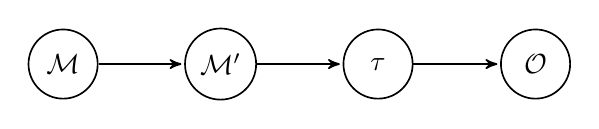
\begin{tikzpicture}[->,>=stealth',shorten >=1pt,auto,node distance=2cm,semithick]
	  \node[state] (A)              {$\mathcal{M}$};
	  \node[state] (B) [right of=A] {$\mathcal{M}'$};
	  \node[state] (C) [right of=B] {$\tau$};
	  \node[state] (D) [right of=C] {$\mathcal{O}$};
	  \path
(A) edge  node {} (B)
(B) edge  node {} (C)
(C) edge  node {} (D)
;
	\end{tikzpicture}
  \end{center}
  \end{scriptsize}
 \caption{\small {\em Bayesian network} representing that model $\mathcal{M}$ is {\em transformable} into a model $\mathcal{M}'$ that produces a trajectory $\tau(\pi,P)$ that (1) reaches the goals in $P$ and (2) it is consistent with $\mathcal{O}(\tau)$.}
\label{fig:net}
\end{figure}

Our approach to formulate the $P(\mathcal{O}|\mathcal{M})$ likelihood is to assess the cost of transforming $\mathcal{M}$ into a model $\mathcal{M'}$ that produces a trajectory $\tau(\pi,P)$ such that: (1) $\tau(\pi,P)$ reaches the goals in $P$ and (2) $\tau(\pi,P)$ is consistent with observation $\mathcal{O}(\tau)$. Figure~\ref{fig:net} shows the {\em Bayesian network} that embodies this procedure. Regarding this network we have the following formulation of the $P(\mathcal{O}|\mathcal{M})$ {\em likelihood}:

\begin{align}
 P(\mathcal{O}|\mathcal{M})=\sum_{\mathcal{M}'}\sum_{\tau} P(\mathcal{M'}|\mathcal{M})P(\tau|\mathcal{M'})P(\mathcal{O}|\tau),
\end{align}

where $\tau$ ranges over all the trajectories consistent with $\mathcal{O}(\tau)$ that can be synthesized with a model $\mathcal{M}'$ and $\mathcal{M}'$ ranges over all the models that can be generated {\em transforming} $\mathcal{M}$.

The exact computation of $P(\mathcal{O}|\mathcal{M})$ with equation (2) is intractable. For most planning problems the set of trajectories consistent with an arbitrary observation can easily be huge, infinite in the case of planning problems without dead-ends~\cite{lesh1995sound}. Even worse, the number of models $\mathcal{M}'$ that can be generated {\em transforming} a given classical planning model $\mathcal{M}$ explodes combinatorially with the number of state variables. Instead, our approach is to estimate of $P(\mathcal{O}|\mathcal{M})$ using an {\em edit distance} referred to \strips\ planning models. {\em Edit distances} are similarity metrics, traditionally computed over {\em strings} or {\em graphs}, which have been proved successful for {\em pattern recognition}~\cite{MasekP80,Bunke97}. In this work, we assess the cost of {\em transforming} $\mathcal{M}$ into $\mathcal{M'}$ computing {\em edit distances} between \strips\ planning models.


\section{Recognition of \strips\ planning models}
\label{sec:asPlanning}

Our formalization of a model recognition task is valid for any planning model but our \emph{edit distance} measure is exclusively for \strips\ models and so we restrict our attention to \strips\texttt{-}compilable planning models\footnote{An edit distance for other planning models is also definable}. Thus, we focus on the recognition of $\mathcal{M}\in M$, where $M$ is a set of \strips\ planning models and $\mathcal{M}$ defines the semantics of the actions through a set of \strips\ action schemata.


\subsection{Well-defined \strips\ action schemata}
\strips\ action schemata provide a compact representation for specifying classical planning models. Figure~\ref{fig:model-example} shows six \strips\ action schemata that shape a particular kind of robot navigation in $N\times N$ grids (no matter the grid size).

{\em A \strips\ action schema} $\xi$ is defined by four lists: A list of {\em parameters} $pars(\xi)$, and three list of predicates (namely $pre(\xi)$, $del(\xi)$ and $add(\xi)$) that shape the kind of fluents that can appear in the {\em preconditions}, {\em negative effects} and {\em positive effects} of the actions induced from that schema.

\begin{definition}[Comparable \strips\ action schemata]
Two \strips\ schemata $\xi$ and $\xi'$ are {\bf comparable} iff $pars(\xi)=pars(\xi')$, i.e, both share the same list of parameters.\footnote{In \strips\ models, $pars(\xi)=pars(\xi')$ implies the number of parameters must be the same. For other planning models that allow object typing, the equality implies that parameters share the same type}
\end{definition}

For instance, we claim that the six action schemata of Figure~\ref{fig:model-example} are {\em comparable} while, for example, the {\small\tt stack(?v1,?v2)} and {\small\tt pickup(?v1)} schemata from a four operator {\em blocksworld}~\cite{slaney2001blocks} are not. Last but not least, we say that two \strips\ models $\mathcal{M}$ and $\mathcal{M}'$ are {\em comparable} iff there exists a bijective function $\mathcal{M} \mapsto \mathcal{M}^*$ that maps every action schema $\xi\in\mathcal{M}$ to a comparable schemata $\xi'\in\mathcal{M'}$ and vice versa.

Let be $\Psi$ the set of {\em predicates} that shape the propositional state variables $F$, and a list of {\em parameters} $pars(\xi)$. The set of elements that can appear in $pre(\xi)$, $del(\xi)$ and $add(\xi)$ of the \strips\ action schema $\xi$ is given by FOL interpretations of $\Psi$ over the parameters $pars(\xi)$. We denote this set of FOL interpretations as ${\mathcal I}_{\Psi,\xi}$. For any of the six action schemata of Figure~\ref{fig:model-example}, the ${\mathcal I}_{\Psi,\xi}$ set contains the same ten elements, ${\mathcal I}_{\Psi,\xi}=${\small\tt\{xcoord($v_1$), xcoord($v_2$), ycoord($v_1$), ycoord($v_2$), q0(), q1(), next($v_1$,$v_1$), next($v_1$,$v_2$), next($v_2$,$v_1$), next($v_2$,$v_2$))\}}.

Despite any element of ${\mathcal I}_{\Psi,\xi}$ can {\em a priori} appear in the $pre(\xi)$, $del(\xi)$ and $add(\xi)$ of schema $\xi$, the space of possible \strips\ schemata is constrained by a set ${\mathcal C}$ that includes:

\begin{itemize}
\item {\em Syntactic constraints}. \strips\ constraints require $del(\xi)\subseteq pre(\xi)$, $del(\xi)\cap add(\xi)=\emptyset$ and $pre(\xi)\cap add(\xi)=\emptyset$. Considering exclusively these syntactic constraints, the size of the space of possible \strips\ schemata is given by $2^{2\times|{\mathcal I}_{\Psi,\xi}|}$. For every action schema in the navigation model of Figure~\ref{fig:model-example} then $2^{2\times 10}=1,048,576$.

\item {\em Domain-specific constraints}. One can introduce domain-specific knowledge to constrain further the space of possible schemata. For instance, in a {\em robot navigation} model like the one in Figure~\ref{fig:model-example}, {\small\tt q0()} and {\small\tt q1()} are exclusive so they cannot hold at the same time in a $pre(\xi)$/$del(\xi)$/$add(\xi)$ list. Further, {\small\tt next($v_1$,$v_1$)} and {\small\tt next($v_2$,$v_2$)} will not appear in any of these lists because the {\tt\small next} predicate codes the {\em successor} function for {\em natural numbers}. These domain-specific constraints reduce further the size of the space of possible action schemata to $2^{2\times 7}=16,384$ (for every schema in the navigation model of Figure~\ref{fig:model-example}).
\end{itemize}

\begin{definition}[Well-defined \strips\ action schemata]
Given a set of {\em predicates} $\Psi$, a list of action {\em parameters} $pars(\xi)$, and set of FOL constraints ${\mathcal C}$, $\xi$ is a {\bf well-defined \strips\ action schema} iff its three lists $pre(\xi)\subseteq {\mathcal I}_{\Psi,\xi}$, $del(\xi)\subseteq{\mathcal I}_{\Psi,\xi}$ and $add(\xi)\subseteq{\mathcal I}_{\Psi,\xi}$ only contain elements in ${\mathcal I}_{\Psi,\xi}$ and they satisfy all the constraints in ${\mathcal C}$.
\end{definition}

We say a planning model $\mathcal{M}$ is {\em well-defined} if all its \strips\ action schemata are {\em well-defined}.

\subsection{Edit distances for \strips\ planning models}
First, we define the two edit \emph{operations} on a schema $\xi$ that belongs to a \strips\ model $\mathcal{M}\in M$:

\begin{itemize}
\item {\em Deletion}. Given $\xi\in\mathcal{M}$, an element from any of the lists $pre(\xi)$/$del(\xi)$/$add(\xi)$ is removed such that the result is a {\em well-defined} \strips\ action schema.
\item {\em Insertion}. Given $\xi\in\mathcal{M}$, an element in ${\mathcal I}_{\Psi,\xi}$ is added to any of the lists $pre(\xi)$/$del(\xi)$/$add(\xi)$ such that the result is a {\em well-defined} action schema.
\end{itemize}

We can now formalize an {\em edit distance} that quantifies how similar two given \strips\ models are. The distance is symmetric and meets the {\em metric axioms} provided that the two edit operations, {\em deletion} and {\em insertion}, have the same positive cost.

\begin{definition}[Edit distance]
  Let $\mathcal{M}$ and $\mathcal{M}'$ be two {\em comparable} and {\em well-defined} \strips\ planning models within the same set of predicates $\Psi$. The {\bf edit distance} $\delta(\mathcal{M},\mathcal{M}')$ is the minimum number of {\em edit operations} that is required to transform $\mathcal{M}$ into $\mathcal{M}'$.
\end{definition}

Since ${\mathcal I}_{\Psi,\xi}$ is a bounded set, the maximum number of edits that can be introduced to an action model is bounded as well. The \textbf{maximum edit distance} of a \strips\ model $\mathcal{M}$ built with predicates $\Psi$ is $\delta(\mathcal{M},*)=\sum_{\xi\in\mathcal{M}} 3\times|{\mathcal I}_{\Psi,\xi}|$ (note that if we consider the set of syntactic constraints then $\delta(\mathcal{M},*)=\sum_{\xi\in\mathcal{M}} 2\times|{\mathcal I}_{\Psi,\xi}|$).

\vspace{0.02cm}

An observation of the execution of a plan generated with an action model $\mathcal{M}$ further constraints the space of possible action schemata of $\mathcal{M}$. The \emph{semantic knowledge} included in the observations introduce a third type of constraints, that we will call {\em observation constraints}, and that can be added to the set $\mathcal{C}$. In addition, {\em observation constraints} allow us to define an edit distance to elicit the value of $P(\mathcal{O}|\mathcal{M})$. It can be argued that the shorter this distance the better the given model explains the given observation.

\begin{definition}[Observation edit distance]
Given a planning problem $P$, an observation $\mathcal{O}(\tau)$ of the execution of a plan that solves $P$ and a \strips\ planning model $\mathcal{M}$ (all defined within the same set of predicates $\Psi$). The {\bf observation edit distance}, $\delta^o(\mathcal{M},\mathcal{O})$, is the minimal edit distance from $\mathcal{M}$ to any {\em comparable} and well-defined model $\mathcal{M}'$ s.t. $\mathcal{M}'$ produces a trajectory $\tau(\pi,P)$ that reaches the goals in $P$ and is {\em consistent} with $\mathcal{O}(\tau)$; \[\delta^o(\mathcal{M},\mathcal{O})=\min_{\forall \mathcal{M}' \rightarrow \mathcal{O}} \delta(\mathcal{M},\mathcal{M}')\]
\end{definition}

$\delta^o(\mathcal{M},\mathcal{O})$ can also be defined through the edition that the observation $\mathcal{O}(\tau)$ requires to fit $\mathcal{M}$. This implies defining {\em edit operations} that modify the observation $\mathcal{O}(\tau)$ instead of the model $\mathcal{M}$~\cite{yang2007learning,SohrabiRU16}. Our definition of {\em observation edit distance} is more practical since the size of ${\mathcal I}_{\Psi,\xi}$ is usually much smaller than $F$ (the number of variables in the action schemata should normally be lower than the number of objects in a planning problem).

\begin{definition}[{\em Closest consistent models}] \label{consistent}
Given a model $\mathcal{M}$, the set $M^*$ of the {\bf closest consistent models} is the set of models $\mathcal{M}'$ that: (1) produce a trajectory $\tau(\pi,P)$ that reaches the goals in $P$ and is {\em consistent} with $\mathcal{O}(\tau)$ and (2) their {\em edit distance} to $\mathcal{M}$ is minimal;
  \[\underset{\forall \mathcal{M}' \rightarrow \mathcal{O}}{\arg\min}\ \delta(\mathcal{M},\mathcal{M}') \]
\end{definition}

\subsection{Approximating the $P(\mathcal{O}|\mathcal{M})$ {\em likelihood}}

Now we we are ready to formulate an informative estimate of the $P(\mathcal{O}|\mathcal{M})$ likelihood for the particular case where models $\mathcal{M}$ are specified with \strips\ action schemata.

\subsubsection{Full observability of the executed plan.} The {\em full observability of the executed plan} is a too strong assumption for {\em model recognition} but it allows us to understand how to build a reasonable estimate of $P(\mathcal{O}|\mathcal{M})$ for the general case.

Under the assumption of {\em full observability}, there is only a single possible trajectory $\tau^*(\pi,P)$ {\em consistent} with the input observation so $P(\mathcal{O}|\tau^*)=1$. Further, there is also a single model that can exactly produce that trajectory (otherwise models are identical, at least, in the actions relevant to the observed trajectory so they can be considered the same model).

Provided that there is a single possible trajectory and a single possible model consistent with the input observation, i.e. $M^*=\{\mathcal{M}^*\}$ then, the probabilities of expression (2) are not added up and expression (1) simplifies to:
\begin{align}
argmax_{\mathcal{M}\in M} P(\mathcal{M^*}|\mathcal{M}) P(\mathcal{M}).
\end{align}
Note that the term $P(\tau|\mathcal{M^*})$ is taken out of the maximization because is independent of the input model $\mathcal{M}\in M$.

\subsubsection{Partial observability of the executed plan.} In a similar way, an approximation to $P(\mathcal{O}|\mathcal{M})$ can be built for the general case, where the executed plan is partially observed. We add the following two assumptions to deal with this general case:

\begin{enumerate}
\item The {\em principle of rationality}: The expectation that intentional agents will tend to choose actions that achieve their goals most efficiently, given their knowledge of the actual world state~\cite{Dennett83}.
\item {\em The best plans for $P$ are unique or have different cost}.
\end{enumerate}

Similar assumptions were taken in previous work for {\em goal recognition}~\cite{ramirez2012plan}. They allow us to assume that the sum in equation (2) is dominated by its largest term, so other terms in the sum are not added up. The largest term corresponds here to the shortest trajectory $\tau^*$ consistent with the observation (which now is assumed to be unique). Note that the more complete is the observation of the plan execution the more accurate is our estimate because it becomes more likely to assume that there is only one trajectory consistent with the input observation.

Again, we have that there is a single model $\mathcal{M}^*$ that can produce a given trajectory $\tau^*$. With this said, both $P(O|\tau^*)$ and $P(\tau^*|\mathcal{M}^*)$ are independent of $\mathcal{M} \in M$ so equation (1) simplifies once again to equation (3) under the previous two assumptions.

\subsubsection{The $P(\mathcal{M^*}|\mathcal{M})$ probability distribution.} $P(\mathcal{M'}|\mathcal{M})$ indicates the probability of {\em transforming} a classical planning model $\mathcal{M}$ into a model $\mathcal{M'}$ by exclusively using the two {\em edit operations} previously defined, {\em deletion} and {\em insertion}.

We know from {\em pattern recognition}~\cite{devroye2013probabilistic} that, if string symbols are uniformly random and independent, the distance of a given string to a fixed string follows a {\em Binomial distribution}. Moreover, the probability that a particular string will be within a distance $D$ is the Cumulative Distribution Function (CDF) for the {\em Binomial distribution}~\cite{wilcox1981review}:
\begin{align}
CDF(D)=\sum_{d=0}^D{{N}\choose{d}}  p^d (1-p)^{N-d}
\end{align}
where $N$ is the length of the string, and $p<0.5$ since we consider that the cost of applying an {\em edit operation} is higher than do not applying it.

With this regard, and considering that \strips\ models $\mathcal{M}\in M$ can be encoded with a propositional representation of fixed length $N$, we formulate the $P(\mathcal{M'}|\mathcal{M})$ probability distribution mapping the distance $\delta(\mathcal{M},\mathcal{M'})$ according to equation:
\begin{align}
P(\mathcal{M'}|\mathcal{M}) = p^d  (1-p)^{N-d}
\end{align}
where $d=\delta(\mathcal{M},\mathcal{M}')$. Likewise we can formulate $P(\mathcal{M^*}|\mathcal{M})$ with this same equation (5) but instead, the parameter $d$ is given by the {\em observation distance}, $d=\delta^o(\mathcal{M},\mathcal{O})$.

In other words, we are modeling the edition of a \strips\ planning model as a {\em Bernoulli process} in which there is a sequence of $N$ independent events representing $N$ binary decisions (the $N$ possible applications of the edition operations) such that for every of these events $P(X=\top)=p$ and $P(X=\perp)=1-p$.



\section{Model Recognition as planning}

This section shows that $\delta^o(\mathcal{M},\mathcal{O})$, and hence an approximation to $P(\mathcal{O}|\mathcal{M})$), can be computed with a compilation-to-planning approach as the one proposed in~\cite{aineto2018learning} (AJO approach hereafter) for learning \strips\ models. The AJO approach receives as input an empty model $\mathcal{M}$, which only contains the headers of the action schemata formed of $\xi=\tup{name(\xi),pars(\xi)}$, and an observation of a plan execution $\mathcal{O}(\tau)$ (extensible to a set of observations), and it returns a model $\mathcal{M'}$ with specification of preconditions and effects of each action schema included in $\mathcal{M}$ such that the validation of $\mathcal{O}(\tau)=\tup{s_0^o,a_1^o,s_1^o \ldots , a_l^o, s_m^o}$ following $\mathcal{M'}$ is successful; i.e., it holds $\rho(s_{i-1},a_i)$ for every observed action of $\mathcal{O}(\tau)$ and $s_i=\theta(s_{i-1},a_i)$ for every observed state of $\mathcal{O}(\tau)$.

In essence, the task $\tup{\mathcal{M},\mathcal{O}}$ of the AJO approach -- learning $\mathcal{M}$ that satisfies $\mathcal{O}$-- can be interpreted as editing the empty action schemata of $\mathcal{M}$ introducing preconditions and effects until $\mathcal{O}$ is validated with the resulting model. We leverage the same idea to compute $\delta^o(\mathcal{M},\mathcal{O})$ with the exception that now our $\mathcal{M}$ is not empty but $\mathcal{M}=\{\xi_1, \ldots, \xi_m\}$, where $\xi_i=\tup{name(\xi_i),pars(\xi_i),pre(\xi_i),add(\xi_i),del(\xi_i)}$, $1 \leq i \leq m$.

Editing/learning the action schemata of $\mathcal{M}$ in the AJO approach is addressed converting the task into a classical planning problem, which is later solved with a planner. The intuition behind this compilation is that a solution plan to the problem is a sequence of: (a) \emph{edit actions} on the schemata of $\mathcal{M}$ to build $\mathcal{M'}$ and (b) \emph{validate actions} that apply $\mathcal{M'}$ in $\mathcal{O(\tau)}$. The adaptation of this compilation scheme for solving $\delta^o(\mathcal{M},\mathcal{O})$ results in a planning problem $P'=\tup{F',A',I',G'}$ whose objective is to determine the preconditions and effects that need to be added or deleted to the action schemata of $\mathcal{M}$ so as to satisfy $\mathcal{O}$. The accomplishment of this task requires therefore a propositional encoding of the components of the action schemata. Specifically:

\begin{itemize}
\item $F'$ contains the necessary fluents to represent the $pre$, $add$ and $del$ of the action schemata. It is a set of \emph{editable fluents} of the type $\{pre\_e\_\xi, del\_e\_\xi, add\_e\_\xi\}_{\forall e\in{\mathcal I}_{\Psi,\xi}}$ such that $e\in{\mathcal I}_{\Psi,\xi}$ is a single element from the set of FOL interpretations of predicates $\Psi$ over the corresponding parameters $pars(\xi)$. Additionally, $F$ also contains fluents to encode the \emph{observation constraints}; that is, fluents to iterate through the $l$ observed actions and $m$ observed states of $\mathcal{O(\tau)}$.
\item $A'$ comprises two types of actions with conditional effects:
    \begin{itemize}
    \item actions for editing $\xi \in \mathcal{M}$ that follow the \emph{syntactic constraints} for well-defined \strips\ action schemata. Hence, $A'$ contains actions for inserting a new precondition $pre\_e\_\xi$ or a new positive effect $add\_e\_\xi$ in $\xi$ when neither $pre\_e\_\xi$, $del\_e\_\xi$ or $add\_e\_\xi$ exist in $\xi$, and actions for inserting a new negative effect when neither $del\_e\_\xi$ or $add\_e\_\xi$ appear in $\xi$ but $pre\_e\_\xi$ does.
    \item actions for applying the new action schemata of the edited model $\mathcal{M'}$ and validating the observed states of $\mathcal{O(\tau)}$. Particularly, the \emph{apply} actions check the preconditions and produce the effects defined by the \emph{editable fluents}.
    \end{itemize}
\item $I'$ encodes the editable fluents $pre\_e\_\xi, del\_e\_\xi$ and $add\_e\_\xi$ that hold in the action schemata of $\mathcal{M}$.
\item $G'$ contains the necessary fluents to check that all the observed actions and states of $\mathcal{O(\tau)}$ are generated correctly following the edited model $\mathcal{M'}$.
    %Here we include the necessary fluents to check the final reached state is consistent with the final state $s_m^o$ of $\mathcal{O(\tau)}$.
\end{itemize}

We now show an example of a solution plan to a planning problem $P'$ that results from compiling a specific task $\tup{\mathcal{M},\mathcal{O}}$. Consider that $\mathcal{M}$ is the model of Figure~\ref{fig:model-example} except that the schema {\tt\small inc-x} is defined without preconditions and its positive/negative effects are swapped wrt Figure~\ref{fig:model-example}. And consider an observation that only contains the initial and final state of Figure~\ref{fig:grid-example}; i.e., $\mathcal{O(\tau)}=\tup{s_0^o,s_m^o}=\tup{(1,1),(3,2)}$. The plan found by a planner to $P'$ is shown in figure~\ref{fig:plan-pdistance}. The first seven steps are the edit actions to \emph{fix} the schema {\tt\small inc-x}; step 07 is a validate action that sets the robot in the initial state $s_0^o=(1,1)$; step 08 applies the action {\tt\small (inc-x 1 2)} and moves the robot one cell to the right to $(2,1)$; steps 09-11 also move the robot one cell to the right; step 11 applies an action that increases coordinate $y$ to an even number, thus moving robot to row $2$; step 12 moves the robot one cell to the left and, finally, action {\tt\small (validate\_1)} checks the robot position is consistent with the final state $s_m^o=(3,2)$.


\begin{figure}
{\tt\tiny
\begin{tabular}{ll}
00 : (insert\_pre\_xcoord\_v1\_inc-x)   & 07 : (validate\_0)\\
01 : (insert\_pre\_next\_v1\_v2\_inc-x) & 08 : (apply\_inc-x 1 2)\\
02 : (insert\_pre\_q0\_inc-x)           & 09 : (apply\_inc-x 2 3)\\
03 : (delete\_del\_xcoord\_v2\_inc-x)   & 10 : (apply\_inc-x 3 4) \\
04 : (delete\_add\_xcoord\_v1\_inc-x)   & 11 : (apply\_inc-y-even 1 2)\\
05 : (insert\_del\_xcoord\_v1\_inc-x)   & 12 : (apply\_dec-x 4 3)\\
06 : (insert\_add\_xcoord\_v2\_inc-x)   & 13 : (validate\_1)
\end{tabular}
}
 \caption{\small A plan for $\tup{\mathcal{M},\mathcal{O}}$ where $\mathcal{M}$ is a modification of the model of Figure \ref{fig:model-example} and $\mathcal{O}$ a partial observation from Figure~\ref{fig:grid-example}.}
\label{fig:plan-pdistance}
\end{figure}


The value of the {\em observation distance} $\delta^o(\mathcal{M},\mathcal{O})$ is given by the number of {\em edit operations} (insertions and deletions) required by $\mathcal{M}$ to be validated in the input observation. In the case of the above example, the distance equals $7$.



\section{Evaluation}
\label{sec:evaluation}

This section presents three different applications of {\em model recognition} and evaluates the empirical performance of {\em model recognition as planning} when addressing the three of them.

In all the experiments we define a set $M$ of different planning models, that share the same state variables but that update these variables according to different action schemata. Then for each model $\mathcal{M}\in M$, we generate {\em partial observations} $\mathcal{O}(\tau)$ of {\em plan trajectories} that were computed with that model. Finally, we apply our {\em model recognition as planning} method to identify which model, among the models in $M$, was actually used for generating a given $\mathcal{O}(\tau)$ observation. For all the experiments, we assume equal prior probabilities, meaning $P(\mathcal{M}) = \frac{1}{|M|}$ for every $\mathcal{M} \in M$. 

To provide a better explanation of the experiments below, we introduce a particular class of $\mathcal{O}(\tau)$ observations. This new class allows us to distinguish between {\em observable} state variables, whose value may come from sensors, and {\em hidden} or {\em latent} state variables that cannot be observed.
\begin{definition}[$\Phi$-observation]
Given a subset of fluents $\Phi\subseteq F$ we say that $\mathcal{O}(\tau)$ is a $\Phi$-observation of the execution of $\pi$ on $P$ iff, for every ${\small 1\leq i\leq m}$, each observed state $s_i^o$ only contains fluents in $\Phi$.
\end{definition}
Therefore the value of variables in $\Phi\subseteq F$ can be {\em observed} while the value of the variables in $F\setminus\Phi$ is {\em hidden}. 

\subsubsection{Reproducibility.} All experiments were run in an Intel Core i5 3.10GHz x 4 16GB of RAM and the classical planner we used to solve the instances that result from the compilation was {\sc Madagascar}~\cite{rintanen2014madagascar} because of its ability to deal with classical planning problems with dead-ends~\cite{lopez2015deterministic}. We set up a timeout of 1000s for the computation of $\delta^o(\mathcal{M},\mathcal{O})$, at which point it is assigned maximum distance. Compilation source code, evaluation scripts and benchmarks are fully available at this anonymous repository {\em } so any experimental data reported in the paper can be reproduced.

\subsection{Recognition of {\em regular automata}.} The first experiment, which doubles as a proof of concept, leverages {\em model recognition as planning} to perform a typical {\em string classification} problem. In this experiment, the system receives (1) the string to classify (the $\mathcal{O}(\tau)$ observation) and (2), a set $M$ of different planning models, where each $\mathcal{M}\in M$ codes a different class (i.e. a different regular automata that accepts any string that belong to the class).

Figure~\ref{fig:regautomatae} illustrates a three-symbol four-state {\em regular automata} for recognizing the $(abc)^+$ language. The {\em input alphabet} is $\Sigma=\{a,b,c\}$, and the machine states are $Q=\{q_0,q_1,q_2,\underline{q_3}\}$ (where \underline{$q_3$} is the only acceptor state). For instance, the execution of the planning model coding the {\em regular automata} defined in Figure~\ref{fig:regautomatae}, and with the input string $abcabc$, produces the following six-action plan {\small $(\langle a,q_0\rangle\rightarrow q_1)$, $(\langle b,q_1\rangle\rightarrow q_2)$, $(\langle c,q_2\rangle\rightarrow \underline{q_3})$, $(\langle a,\underline{q_3}\rangle\rightarrow q_1)$, $(\langle b,q_1\rangle\rightarrow q_2)$, $(\langle c,q_2\rangle\rightarrow \underline{q_3})$}.

\begin{figure}
  \begin{scriptsize}
  \begin{center}
	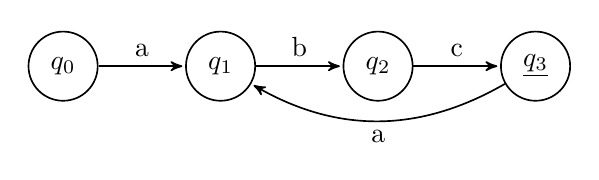
\begin{tikzpicture}[->,>=stealth',shorten >=1pt,auto,node distance=2cm,semithick]
	  \node[state] (A)              {$q_0$};
	  \node[state] (B) [right of=A] {$q_1$};
	  \node[state] (C) [right of=B] {$q_2$};
	  \node[state] (D) [right of=C] {\underline{$q_3$}};
	  \path
(A) edge  node {a} (B)
(B) edge  node {b} (C)
(C) edge  node {c} (D)
(D) edge [bend left]  node {a} (B)
;
	\end{tikzpicture}
  \end{center}
  \end{scriptsize}
 \caption{\small Three-symbol four-state {\em regular automata} for recognizing the $(abc)^+$ language (\underline{$q_3$} is the acceptor state).}
\label{fig:regautomatae}
\end{figure}

%Note that the the string to classify is a {\em $\Phi$-observation} since it does not contain any information about the structure of the possible regular automata. This means that $\mathcal{O}(\tau)$ is a $\Phi$-observation where fluents representing the internal machine state are unknown and the applied transitions (actions) are unobserved.

In this experiment, $M$ comprises 5 planning models representing different regular automata defined with 5 states and a 4-symbol alphabet. The five regular languages defined by these five automata are the following:
\begin{itemize}
	\item $\mathcal{L}$1: $a^+(b|c)d(dd)^*a$
	\item $\mathcal{L}$2: $bd(abd)^*cd^*c^+$
	\item $\mathcal{L}$3: $d^*c(ac)^*db^*ac^*b^+$
	\item $\mathcal{L}$4: $(cc)^+bd(abd)^*$
	\item $\mathcal{L}$5: $(d|a)a(ba)^*c^+d(dc^*d)^*$
\end{itemize}

For each regular language, we generated $20$ random strings, $\mathcal{O}(\tau)$ observations, of length 20 to 30 for a total of 100 strings. More precisely observations $\mathcal{O}(\tau)$ are $\Phi$-observations where: the applied automata transitions and the fluents representing the internal automata state are unobserved. Table \ref{tab:conf_matrix} shows the {\em confusion matrix} resulting from classifying these 100 strings with {\em model recognition as planning}. In this matrix, rows represent the actual class and columns the class predicted by our {\em model recognition as planning} approach. Even though we are using a suboptimal classical planner, we can see that the class for all the 100 input strings was correctly recognized. These results proof the suitability of {\em model recognition as planning} for classification tasks where classes are given as generative planning models and examples are sequence of observations.

\begin{table}
	\centering
	\begin{tabular}{c|c|c|c|c|c}
		& $\mathcal{L}$1 & $\mathcal{L}$2 & $\mathcal{L}$3 & $\mathcal{L}$4 & $\mathcal{L}$5\\ \hline
		$\mathcal{L}$1 & 20 & 0 & 0 & 0 & 0 \\
		$\mathcal{L}$2 & 0 & 20 & 0 & 0 & 0 \\
		$\mathcal{L}$3 & 0 & 0 & 20 & 0 & 0 \\
		$\mathcal{L}$4 & 0 & 0 & 0 & 20 & 0 \\
		$\mathcal{L}$5 & 0 & 0 & 0 & 0 & 20 \\
	\end{tabular}
	\caption{Confusion matrix for {\em regular automata recognition}.}
	\label{tab:conf_matrix}
\end{table}



\subsection{Recognizing failures in a non-deterministic {\em blocksworld}}
With this second experiment we aim to validate the assumptions underlying our approximation of the $P(\mathcal{O}|\mathcal{M})$ likelihood. These assumptions being that the agent acts rational, so $P(\mathcal{O}|\mathcal{M})$ is dominated by the shortest trajectory that explains the observation, and that there exists a single such trajectory.

In this particular experiment we assume that the length of the trajectory is known (to force the explanation to be optimal) and hence, measure the {\em  accuracy} of our approximation of the $P(\mathcal{O}|\mathcal{M})$ likelihood across different degrees of observability. More precisely, we assume that at least one literal is observed at every state so the length of the plan trajectory is fixed by the observation. 

The input observations $\mathcal{O}(\tau)$ come from a non-deterministic {\em blocksworld} in which some of the executed actions failed. We considered failures of three kinds:
\begin{itemize}
	\item $\mathcal{F}$1: the execution of a {\tt\small stack} action fails causing no effect.
	\item $\mathcal{F}$2: {\tt\small unstack} fails dropping the block to unstack on the table.        
	\item $\mathcal{F}$3: {\tt\small unstack} fails doing nothing.
\end{itemize}
The input models in $M$ are then three different {\em extended} 4-operator {\em blocksworlds} such that each of these models includes an additional action schema that encodes one of the three failures above. This means that failures are identified by finding the model that explains the best the input observation. 

Figure \ref{fig:blocks_acc} shows the {\em accuracy} of our approach when identifying failures over 30 different observations. {\em Accuracy} is defined as the number of correct predictions over all predictions made while the {\em degree of observability} indicates the probability of observing a literal in an intermediate state. The figure showcases a positive trend proving that the more complete the observations are the more accurate our estimation becomes. The overall high accuracy validates our assumption that the trajectory that better explains the observation is the shortest one. %We limited the failures to be of one kind per observation however, it would be possible to recognize different combinations of them. 

\begin{figure}
	\centering
	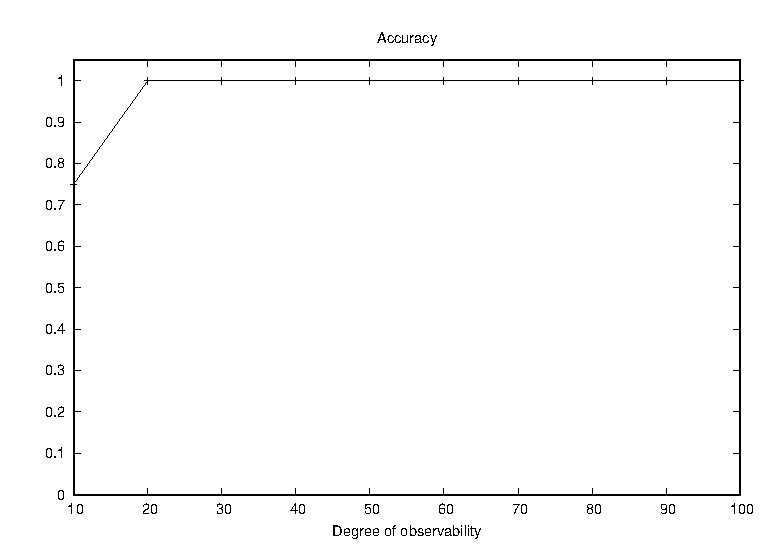
\includegraphics[width=0.9\linewidth]{figures/blocks.eps}
	\caption{Accuracy for the recognition of failures in a non-deterministic {\em blocksworld}.}
	\label{fig:blocks_acc}
\end{figure}



\subsection{Recognition of navigation policies}
Again, this experiment evaluates the accuracy of {\em model recognition as planning} to identify the model that generated each observation under different {\em degrees of observability}. The novel aspect of this experiment is that now, we do not guarantee that observed states contain at least one literal, meaning that some intermediate states may be missing. Therefore, in this new scenario more than a single action may be required to reach one observed state from another.

In this experiment the planning models given in $M$ represent different navigation models for $N\times N$ grids. In particular, we took a {\em classical navigation model} with actions {\tt\small up, down, right, left} (to move one cell in each of these four directions) and extend it to define 8 different navigation policies with respect to these additional state variables {\tt\small \{(q0), (q1), (min ?v), (max ?v)\}}. An example is the navigation policy, shown in Figure~\ref{fig:model-example}. This policy allows to move right when $q_0$ holds while it allows to move left when $q_1$ holds, producing a zig-zag pattern when visiting all the cells of $N\times N$ grids.

Note that all navigation policies are at a maximum distance of just 4 editions from the base {\em classical navigation model} that can move in any direction at any given state. This aspect constrains the discriminating power of the $P(\mathcal{O}|\mathcal{M})$ likelihood, and added to the low observability of the states, produces a touchstone for {\em model recognition as planning}.

On the other hand we generated observations from 8 different trajectories, one for each of the 8 previous planning models. The trajectories depict paths followed by each navigation policy to solve the planning problem of {\em visiting all} cells in a $5\times 5$ grid. As in the previous experiments, observations contain no actions and here, for each observed state, only the values of the fluents encoding the {\em x and y coordinates} of the agent are known (i.e. $\Phi =$\{{\small\tt xcoord, ycoord}\}).

Figure \ref{fig:navigation_acc} shows the classification {\em accuracy} achieved by {\em model recognition as planning} with respect to a range of degrees of observability, from 0\% to 100\% with 10\% increments. In this experiment we included the 0\% case which corresponds to observations where only the initial and final states are observed. The figure shows that for 0\% observability we were unable to unmistakably identify the generating navigation policies, but starting from 10\% we start to correctly classify half of the observations. Accuracy stabilizes after 40\% observability in the range 0.875 to 1 which means that, at most, only 1 observation of the 8 was not correctly classified.

\begin{figure}
	\centering
	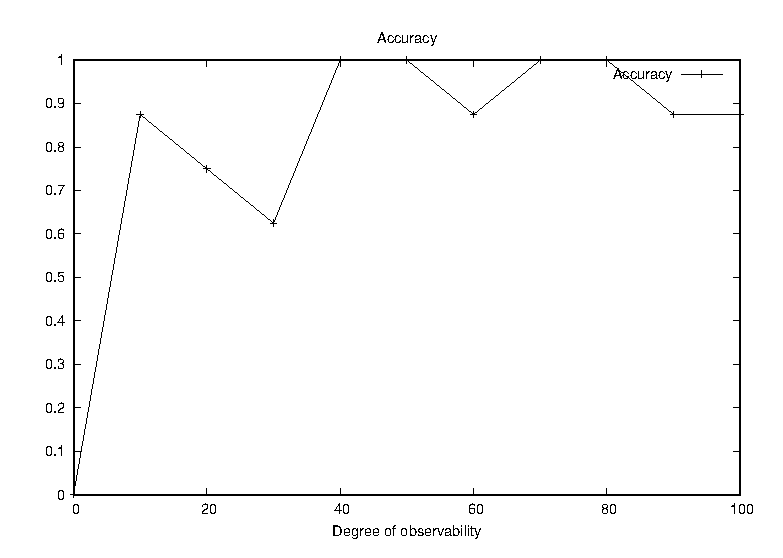
\includegraphics[width=0.9\linewidth]{figures/navigation.eps}
	\caption{Classification accuracy for the recognition of navigation models.}
	\label{fig:navigation_acc}
\end{figure}



\section{Related work}
\label{sec:related}
An interesting research line related with {\em model recognition} is {\em model reconciliation}~\cite{ChakrabortiSZK17}. In {\em model reconciliation} model edition is used to conform the PDDL models of two different agents, or the model of an agent with a given {\em annotated model}~\cite{sreedharan2018handling}, and with respect to a fully observed {\em optimal plan} computed using one of the models. It can be thought that {\em model recognition} conforms every input model $\mathcal{M}$ in the $M$ set with another model $\mathcal{M}'$ s.t. it is {\em consistent} with a partial observation of a plan execution. Note however that in the {\em model recognition} task, the model $\mathcal{M}'$ is not given as input and instead, this model $\mathcal{M}'$ is computed for every $\mathcal{M}\in M$. Further, {\em model recognition as planning} shows that the probability of an input planning model to explain a partial observation of a plan execution (that contains no information of the applied actions and where intermediate states may be incomplete or even missing) can be estimated with an off-the-shelf classical planner.

Once the planning model of the observed agent is recognized, then the model-based machinery for automated planning becomes fully applicable. Of course, this includes the current approaches for {\em goal recognition}~\cite{ramirez2012plan}, {\em goal recognition design}~\cite{KerenGK14} and {\em counter-planning}~\cite{pozanco2018counterplanning} that require to have a model, in advance and fixed, of the observed agent. Last but not least, our approach allows to predict the future actions of an observed agent whose behavior is not ruled by a deliberative planning process that aims to achieve certain goals. As an example, our experiments show that {\em model recognition} is suitable for anticipating the actions of agents that are ruled by the execution of fixed programs or finite state machines, such as a {\em regular automata}.  

%Last but not least, previous work on the learning of \strips\ action models also defined semantic error metrics to quantify the errors of a model with respect to the observation of a plan execution~\cite{yang2007learning}. Our approach for quantifying this error is based on the definition of a edit distance for the model which allow us to not accumulate the repetition of errors coming from the the same model flaw.

\section{Conclusions}
\label{sec:conclussions}
This paper formalized the {\em model recognition} task and proposed, {\em model recognition as planning}, a method built on top of off-the-shelf classical planning algorithms to estimate the probability of a \strips\ model to produce a partial observation of a plan execution. The paper shows the effectiveness of {\em model recognition as planning} in a set of \strips\ models encoding different kinds of {\em automata}. {\em Model recognition as planning} succeeds to identify the executed automata despite the internal machine state or actual applied transitions, are unobserved.






%Remarkably, the extension of this piece of work to the FOND planning setting~\cite{muise2012improved} is straightforward by simply considering the {\em all-outcomes} determiniztion of the actions with non-determinitic effects~\cite{yoon2007ff}. An interesting research direction is however to understand how to apply our approach to planning models where the planning models include actions with probabilistic effects~\cite{younes2005first}.

\newpage

\bibliographystyle{aaai}
\bibliography{planlearnbibliography}

\end{document}
